% Number 690
% pTM 2D Algebra Units Vectors
% Golf ball hit - graphical, 2D
% MIT/JG

% Watermark
\AddToShipoutPicture*{\BackgroundPic}

\addtocounter {ProbNum} {1}

\begin{floatingfigure}[r]{.32\textwidth}
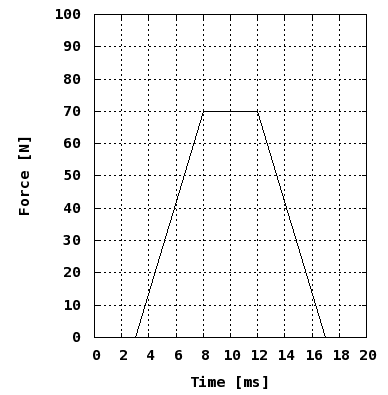
\includegraphics[scale=.5]{/Users/jgates/desktop/latex/pics/golfballgraph}
\end{floatingfigure}
 
{\bf \Large{\arabic{ProbNum}}} A golf ball $(45~g)$ is hit with a club from a tee. The plot shows the force on the ball as a function of time in milliseconds. The golf club's face is inclined so that the ball leaves the club moving 55 degrees above the horizontal.

\bigskip
How far does the golf ball go?\paragraph{}
\noindent
\vfill

What effect (be precise) would decreasing the golf ball's mass by $10\%$ have on the time that the ball spends in the air?
\vfill
%\hfill 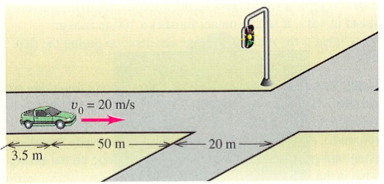
\includegraphics[scale=.85]{/Users/jgates/desktop/latex/pics/redlight.png}
\newpage